%%% LaTeX Template: Two column article
%%%
%%% Source: http://www.howtotex.com/
%%% Feel free to distribute this template, but please keep to referal to http://www.howtotex.com/ here.
%%% Date: February 2011

%%% Preamble
\documentclass[	DIV=calc,%
paper=a4,%
fontsize=12pt,%
onecolumn]{scrartcl}	 					% KOMA-article class

\usepackage{lipsum}													% Package to create dummy text
\usepackage[brazil]{babel}										% English language/hyphenation
\usepackage[protrusion=true,expansion=true]{microtype}				% Better typography
\usepackage{amsmath,amsfonts,amsthm}					% Math packages
\usepackage[pdftex]{graphicx}									% Enable pdflatex
\usepackage[svgnames]{xcolor}									% Enabling colors by their 'svgnames'
\usepackage[hang, small,labelfont=bf,up,textfont=it,up]{caption}	% Custom captions under/above floats
\usepackage{epstopdf}												% Converts .eps to .pdf
\usepackage{subfig}													% Subfigures
\usepackage{booktabs}												% Nicer tables
\usepackage{fix-cm}													% Custom fontsizes
\usepackage[utf8]{inputenc}
\usepackage[top=2.5cm, bottom=2.5cm, left=2.5cm, right=2.5cm]{geometry}
\usepackage[ddmmyyyy]{datetime}
\addto\captionsenglish{%
	\renewcommand\tablename{Tabela}
	\renewcommand\figurename{Figura}
} 



%%% Custom sectioning (sectsty package)
\usepackage{sectsty}													% Custom sectioning (see below)
\allsectionsfont{%															% Change font of al section commands
	\usefont{OT1}{phv}{b}{n}%										% bch-b-n: CharterBT-Bold font
}

\sectionfont{%																% Change font of \section command
	\usefont{OT1}{phv}{b}{n}%										% bch-b-n: CharterBT-Bold font
}



%%% Headers and footers
\usepackage{fancyhdr}												% Needed to define custom headers/footers
\pagestyle{fancy}														% Enabling the custom headers/footers
\usepackage{lastpage}	

% Header (empty)
\lhead{}
\chead{}
\rhead{}

\lfoot{\footnotesize \texttt{Cabeamento estruturado} \textbullet ~Juushin SA}


\cfoot{}
\rfoot{\footnotesize página \thepage\ de \pageref{LastPage}}	% "Page 1 of 2"
\renewcommand{\headrulewidth}{0.0pt}
\renewcommand{\footrulewidth}{0.4pt}



\usepackage{lettrine}
\newcommand{\initial}[1]{%
	\lettrine[lines=3,lhang=0.3,nindent=0em]{
		\color{DarkGoldenrod}
		{\textsf{#1}}}{}}



\usepackage{titling}															% For custom titles

\newcommand{\HorRule}{\color{DarkGoldenrod}%			% Creating a horizontal rule
	\rule{\linewidth}{1pt}%
}

\pretitle{\vspace{-30pt} \begin{flushleft} \HorRule 
		\fontsize{50}{50} \usefont{OT1}{phv}{b}{n} \color{DarkRed} \selectfont 
	}
	
	
	
	\title{Projeto de cabeamento estruturado para Juushin SA}					
	
	
	
	\posttitle{\par\end{flushleft}\vskip 0.5em}

\preauthor{\begin{flushleft}
		\large \lineskip 0.5em \usefont{OT1}{phv}{b}{sl} \color{DarkRed}}
	\author{Fernando Rocha }  	% Author name goes here
	
	
	\postauthor{\footnotesize \usefont{OT1}{phv}{m}{sl} \color{Black} 
		\\Universidade Tecnológica Federal do Paraná - Câmpus Cornélio Procópio 								% Institution of author
		\par\end{flushleft}\HorRule}

\date{}																				% No date




%%% Begin document
\begin{document}
	\maketitle
	\thispagestyle{fancy} 	
	\thispagestyle{empty}		% Enabling the custom headers/footers for the first page 
	
	\initial{E}\textbf{ste projeto tem como propósito apresentar uma estrutura de cabeamento para uma empresa fictícia, consolidando assim o conhecimento adquirido na disciplina de cabeamento estruturado.
		O resumo será descrito no formato texto e em forma de um mapa mental/conceitual conforme figura \ref{fig4}.}
	
	
	\begin{figure}
		\centering
		
\includegraphics{utfpr}
	\end{figure}
	
	\vspace{2cm}
	\centerline{\textit{\textbf{\today}}}
	
	\clearpage
	\renewcommand*\listfigurename{Lista de figuras}
	\listoffigures
	
	\renewcommand*\listtablename{Lista de tabelas}
	\listoftables
	
	
	
	
	\clearpage
	\renewcommand{\contentsname}{Sumário}
	\tableofcontents
	\clearpage
	
	
	\section{Introdução}
	A Juushin SA é uma empresa que atua no área de serviços. Recentemente constituída, ainda não se encontra completamente estabelecida e, por isso, o projeto de cabeamento estruturado para essa empresa iniciará do zero. A Juushin SA conta com um quadro de 25 pessoas, sendo 9 que atuam na sede da empresa; 3 equipes de 5 pessoas, mais 1 Supervisor de equipe que atuam fora da sede. Atualmente a empresa está mudando sua sede e portanto, todo cabeamento será configurado a partir deste projeto.
	
	\subsection{Benefícios}
	
	O planejamento de um sistema de cabeamento traz consideráveis benefícios às empresas que o adotam:
	\begin{itemize}
		\item Unifica a estrutura de dados, voz e vídeo reduzindo custos com manutenção e necessidade de atualização.
		\item Menor propensão a falhas, interrupções e interferências.
		\item Uma estrutura centralizada torna as alterações, que por ventura precisem ser feitas, mais rápidas e eficientes.
		\item Diminui drasticamente a inatividade do sistema, pois o diagnóstico de problemas é mais fácil que em uma rede não estruturada.
		\item O cabeamento estruturado tem maior durabilidade, pois sofre menos manipulação e tem melhor acondicinamento. 
	\end{itemize}
	\subsection{Organizações Envolvidas}
	\begin{table}[h!] % coloque h! para forcar a posicao
		\centering
		\caption{Oraganizações}
		\label{tab1} %com este label vc faz referencia no texto
		\begin{tabular}{|l|l|l|l|l|}
			\hline
			\multicolumn{1}{|c|}{\textbf{Empresa}} & \multicolumn{1}{c|}{\textbf{Serviço}} & \multicolumn{1}{c|}{\textbf{Responsável}} \\ \hline
			Copel Telecom                          & Provedor de Internet 1              & Mévio \\ \hline
			NET                                         & Provedor de Internet 2              & Tício \\ \hline
			BH Construtora                              & Piso e Instalação              & Caio\\ \hline
		\end{tabular}
	\end{table}
	
	\begin{itemize}
		\item os passivos de rede atuais:path panels, cabos, etc..;
		\item as principais reclamações dos usuários. Qual o principal motivo da reestruturação? Efetue uma pesquisa junto aos colaboradores para determinar quais problemas a rede apresenta.
		\item Observações. Analise a rede e verifique se há estruturas que não se enquadram nas normas ou que indicam suspeita de problemas.
	\end{itemize}
	
	\section{Requisitos}
	Crie uma enumeração dos requisitos do projeto.
	\begin{itemize}
		\item Padronizar toda a estrutura de rede.
		\item Identificação dos os cabos.
		\item Separação entre o cabeamento de rede e o cabeamento elétrico.
		\item Atender demanda atual e futuras expansões.				
	\end{itemize}	
	
	\section{Usuários e Aplicativos}
	Atualmente a empresa tem como usuários seus 25 colaboradores mais seus clientes que fazem uso da rede wireless. Com a crescente demanda por serviços este número pode aumentar nos próximos anos, por isso é importante que o projeto preveja uma possível expansão da rede atual.
	
	
	\subsection{Usuários}
	\begin{itemize}
		\item Diretores: 3;
		\item Atendentes: 2;
		\item Administrativo: 4;
		\item Membros das Equipes: 15;
		\item Clientes: até 20;
	\end{itemize}
	\subsection{Aplicativos}
	\begin{itemize}
		\item Sistema ERP: 3;
		\item Pacote Office: 9;
		\item Programa de Vendas: 4;
	\end{itemize}
	
	\section{Estrutura predial existente}
	
	Explique aqui a planta física dos prédios
	Pode ser anexada, em escala ou não.
	
	Deve conter uma descrição geral, indicando a possível distância entre os pontos de rede e restrições de instalação.
	%inicio dos comandos para criar uma nova pagina A3 horizontal
	\clearpage
	\KOMAoptions{paper=a3, paper=landscape, DIV=20}
	\recalctypearea
	
	\begin{figure}
		%	\centering
		\noindent\makebox[\textwidth][c]{
			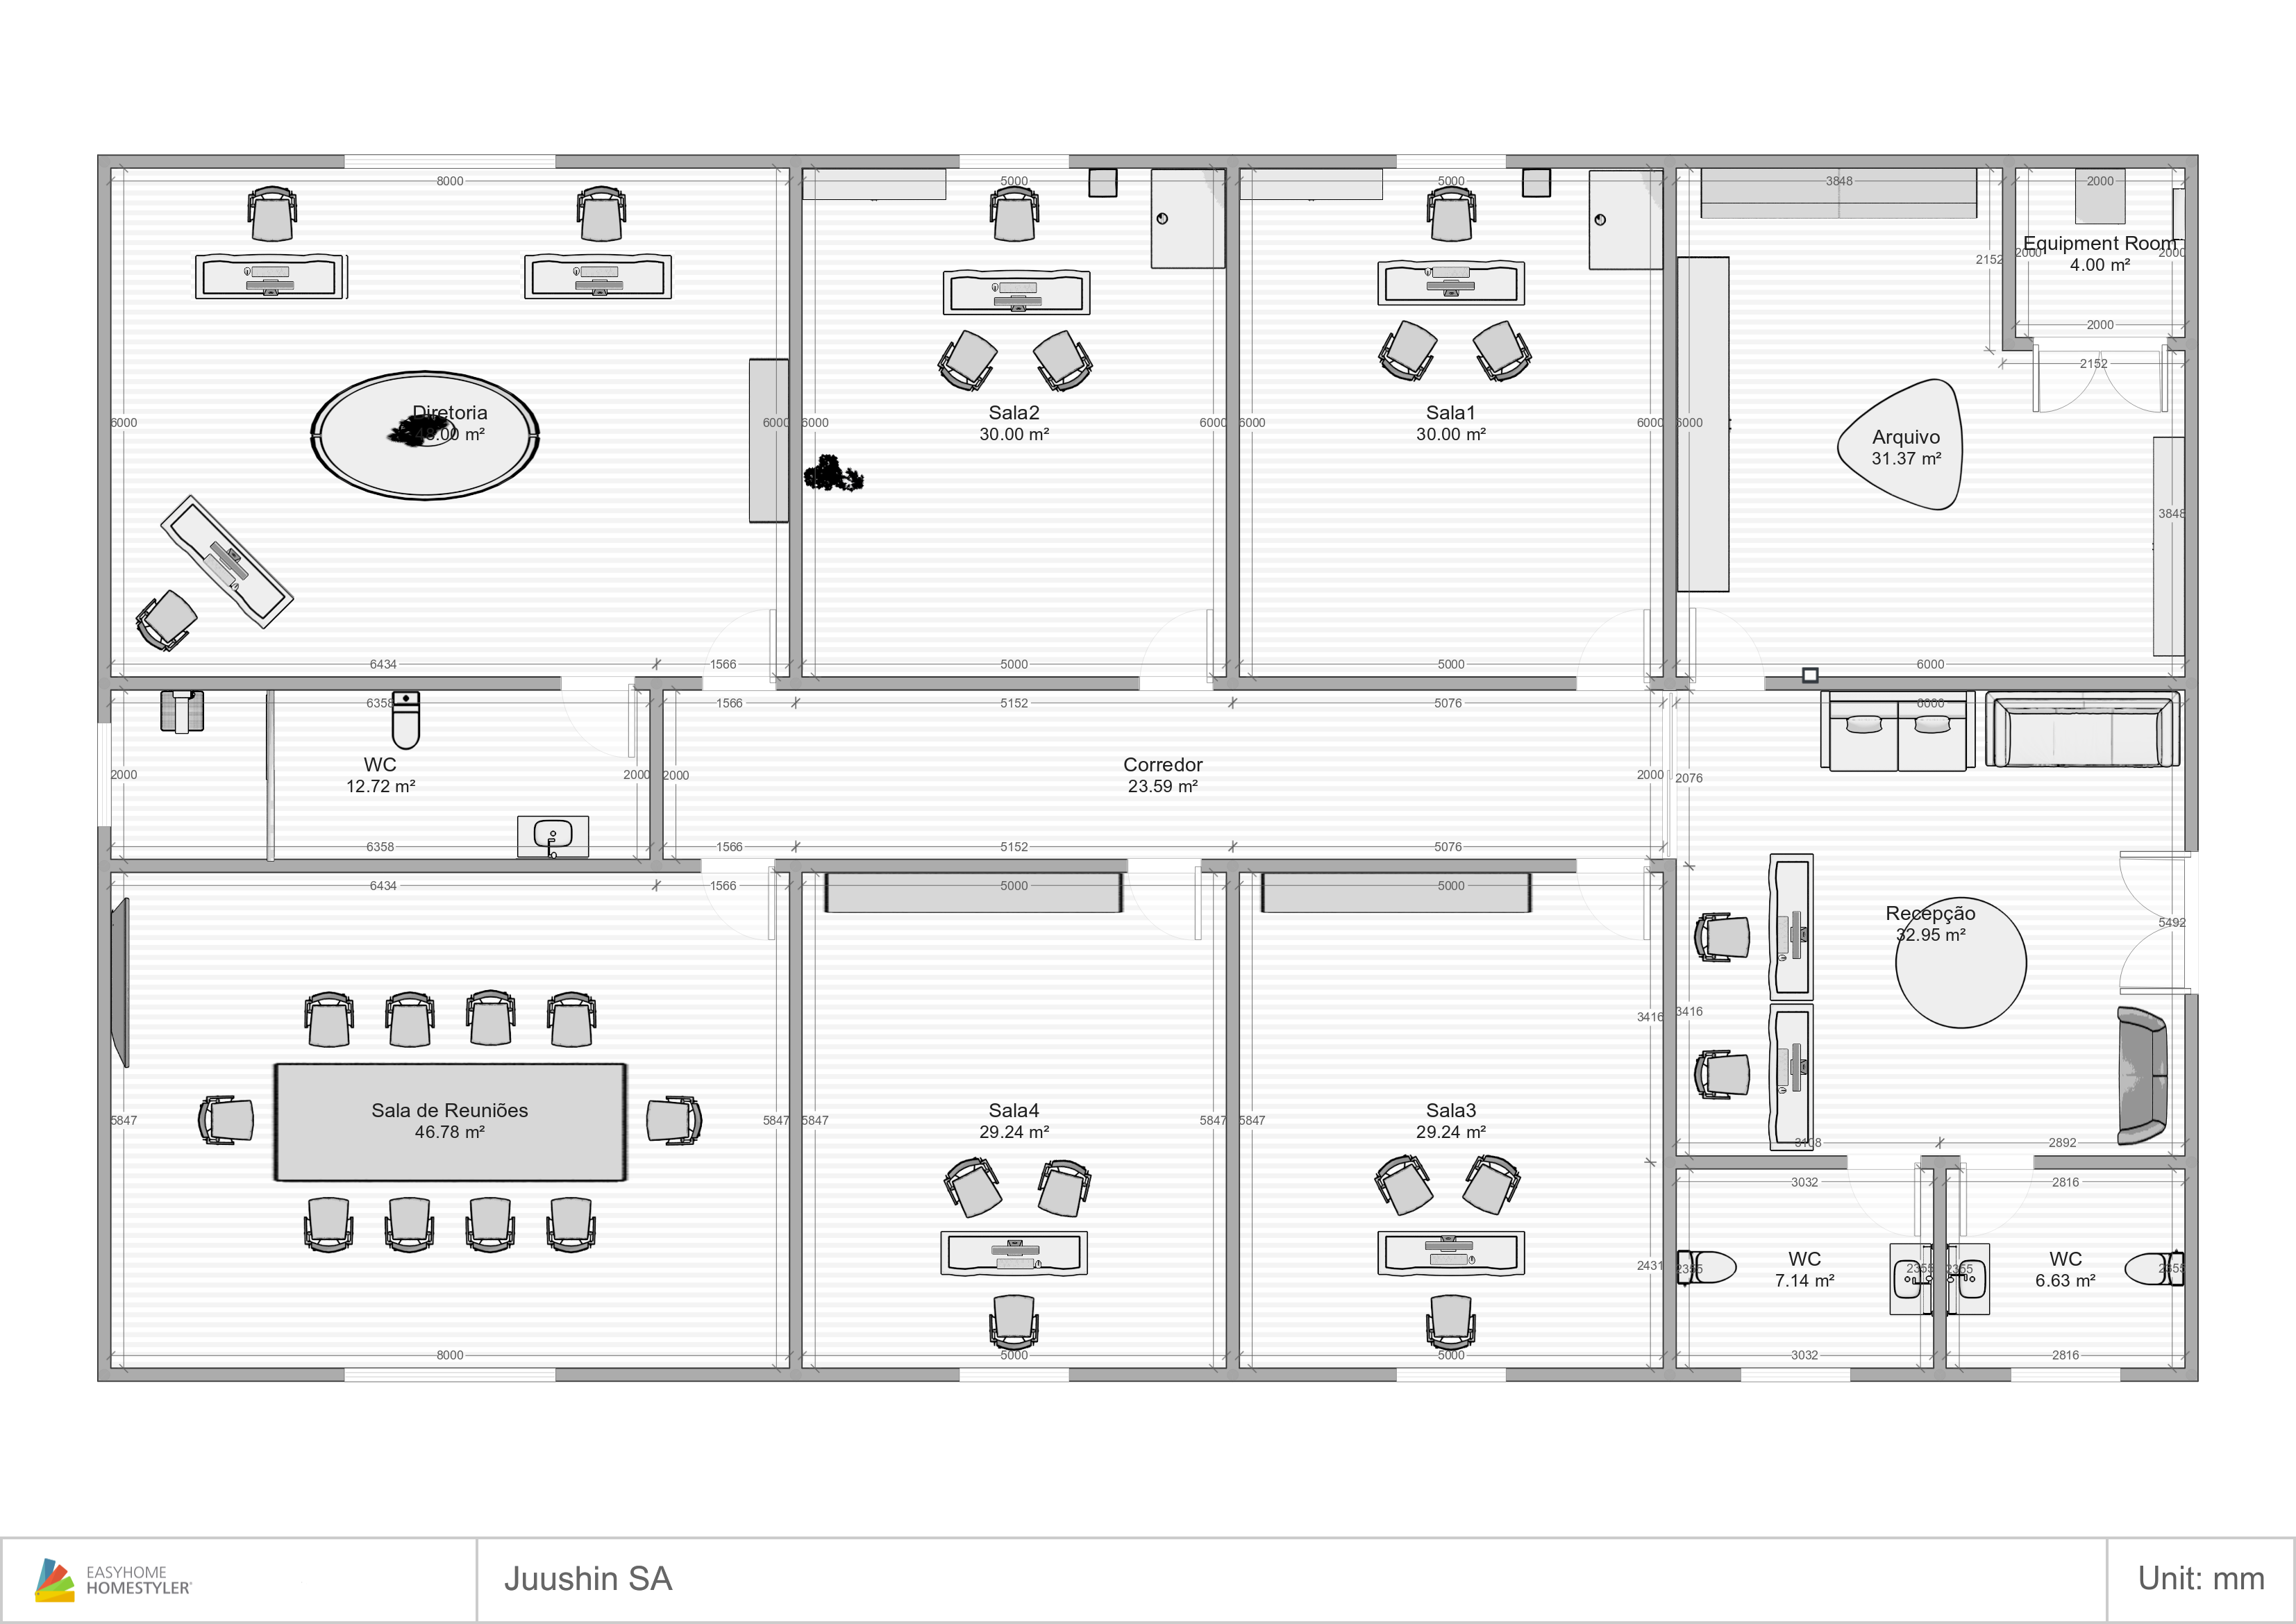
\includegraphics[width=\textwidth]{fig1}
		}
		\caption{Planta física}
		\label{fig1}
	\end{figure}
	
	%Retornar ao formato A4
	\clearpage
	\KOMAoptions{paper=a4, paper=portrait, DIV=calc}
	\recalctypearea
	%-- reinicio em A4 
	\section{Planta Lógica - Elementos estruturados}
	
	\subsection{Estado atual}
	Deve ter a planta atual, se for o caso
	
	\subsection{Topologia}
	Proposta futura, proposta após implantação.
	Deve conter o diagrama da rede. Atente-se a redundância  e ligações truncadas.
	Deve explicar todos termos e componentes utilizados nestas plantas. Por exemplo: entrance facility, work area, horizontal cabling, etc..
	
	Todos os elementos das figuras devem ser explicados. 
	Crie esboço da configuração dos racks e brackets. Explique cada um dos componentes. Você pode criar uma tabela contendo figuras dentro, ou criar uma tabela e incluí-la como imagem. Por exemplo, verifique a tabela \ref{tab1}.
	
	\begin{table}[h!]
\centering
\caption{Exemplo de tabela explicativa}
\label{tab4}
\begin{tabular}{|l|l|l|}
\hline
\multicolumn{3}{|l|}{Figura na Tabela} \\ \hline
1        & Rack          & \includegraphics[scale=0.2]{fig6}        \\ \hline
2        & Rack 2        & \includegraphics[scale=0.2]{fig6}        \\ \hline
\end{tabular}
\end{table}
	
	\subsection{Encaminhamento}
	Eletrodutos, calhas, e qualquer material em que os cabos serão alojados/alocados.
	
	\subsection{Memorial descritivo}
	
	Relacione todos os equipamentos passivos que serão utilizados, tipo, fabricante, quantidade.
	
	\subsection{Identificação dos cabos}
	Explique como os cabos serão identificados em seu projeto. Coloque uma relação dos cabos instalados e identificados.
	
	\section{Implantação}
	Estabeleça um cronograma de implantação:
	Remoção de equipamentos existentes (destino para descarte), instalação dos condutores, instalação dos cabos, 
	identificação dos cabos, montagem dos racks, certificação, etc... Crie atividades e estabeleça o tempo de execução. Se for um projeto real, indique também quais os responsáveis pela execução do projeto e de cada uma das etapas.
	
	Defina marcas (e padrões) e fornecedores se for o caso. Atenção a contratados e subcontratados para a realização das atividades. Estabeleça a responsabilidade de execução da atividade e também da validação dela.
	
	Utilize algum software para gerear o cronograma. Excel,etc. O fundamental é dividir em etapas, descrever e estimar o tempo de cada uma delas.
	
	Segue uma relação de ferramentas:
	http://asana.com/, 
	https://trello.com/, 
	http://www.ganttproject.biz/, 
	http://www.orangescrum.org/. 
	
	\section{Plano de certificação}
	Quais seriam as etapas para a certificação? 
	Quais os locais e horários para execução da certificação na rede? Toda rede será certificada?
	Como os testes seriam executados?
	Quais relatórios de certificação serão (ou deveriam ser) entregues? 
	
	\section{Plano de manutenção}
	
	Revisões periódicas na rede, emissão de certificados para novos pontos.
	
	\subsection{Plano de expansão}
	Existe um plano de expansão? Quantos novos pontos poderão ser acrecidos na rede, antes de migração de equipamentos na camada 2? Se houver expansão, quais equipamentos deverão ser direcionados para as estremidades da rede? 
	
	\section{Risco}
	Enumerar e explicar os riscos do projeto.
	
	\section{Orçamento}
	Crie uma relação de orçamentos baseado na seções anteriores.
	
	\section{Recomendações}
	Observações e recomendações para o cliente.
	
	\section{Referências bibliográficas}
	Utilize o mendley, o jabref ou diretamente o bibtex para gerenciar suas referências biliográficas. As referências são criadas automaticamente de acordo com o uso no texto.
	
	Exemplo: Redes de computadores, segundo \cite{t2013} é considerada..... Já \cite{kurose2010} apresenta uma versão...
	
	Analisando os pressupostos de \cite{ref3} e \cite{ref4} concluimos que....
	
	
	\renewcommand\refname{} %%Referências bibliográficas}  
	\bibliographystyle{ieeetr}
	\bibliography{referencias}  
	
	%% ***********************************************************************
	%% === remover daqui =====================================================
	%% ***********************************************************************
	=================================================
	\section{Elementos textuais - Alguns exemplos}
	
	Esta seção apresenta exemplos de elementos textuais. \textbf{Remova-a da versão final do texto}.
	
	
	\subsection{Colocar elementos em itens}
	
	Texto antes da lista
	
	\begin{itemize}
		\item First item in a list 
		\item Second item in a list 
		\item Third item in a list
	\end{itemize}
	
	\subsubsection{Uma subseção de terceiro nivel}
	
	Exemplo de uma subseção
	
	\subsection{Tabelas}
	
	Utilize o site http://www.tablesgenerator.com/ para elaborar as tabelas de seu trabalho.
	Para adicionar uma tabela utilize: a tag input, passando o arquivo da tabela como parametro
	
	\begin{table}[h!] % coloque h! para forcar a posicao
\centering
\caption{Modifique a legenda e crie um label}
\label{tab2} %com este label vc faz referencia no texto
\begin{tabular}{|l|l|l|l|l|}
\hline
\multicolumn{1}{|c|}{\textbf{Este é um exemplo de tabela}} & \multicolumn{2}{c|}{\textbf{C1}} & \multicolumn{2}{c|}{\textbf{C2}} \\ \hline
Você pode criar a tabela no excel                          & 1              & 2               & 3               & 4              \\ \hline
Exportar para CSV                                          & 5              & 6               & 7               & 8              \\ \hline
E importar no Table Generator                              & 9              & 10              &                 &                \\ \hline
\multicolumn{5}{|c|}{\textit{Gere o tex, e adicione em seu arquivo}}                                                             \\ \hline
\end{tabular}
\end{table}
	
	Dentro do arquivo você deve definir o label e pode utilizá-lo para referenciar. Exemplo:
	Na tab \ref{tab1} temos a relação de ....
	
	
	Você também pode modificar a tabela manualmente, incluindo, por exemplo h! dentro de sua definição. Veja no exemplo tab2.tex
	
	\subsection{Figuras}
	
	As figuras podem ser no formato PDF, JPG, PNG. Você pode referenciá-las da mesma maneira que tabelas. Exemplo: A figura \ref{fig6} apresenta.....
	
	Não se preocupe o local em que a figura será renderizada em seu texto. Preocupe-se em criar referência para ela, ou seja, toda figura e tabela deve conter pelo menos uma referência no texto.
	
	\begin{figure}
		\centering
		\includegraphics[width=\textwidth]{fig6}
		\caption{Exemplo de figura com escala horizontal}
		\label{fig6}
	\end{figure}
	
	
	\begin{figure}
		\centering
		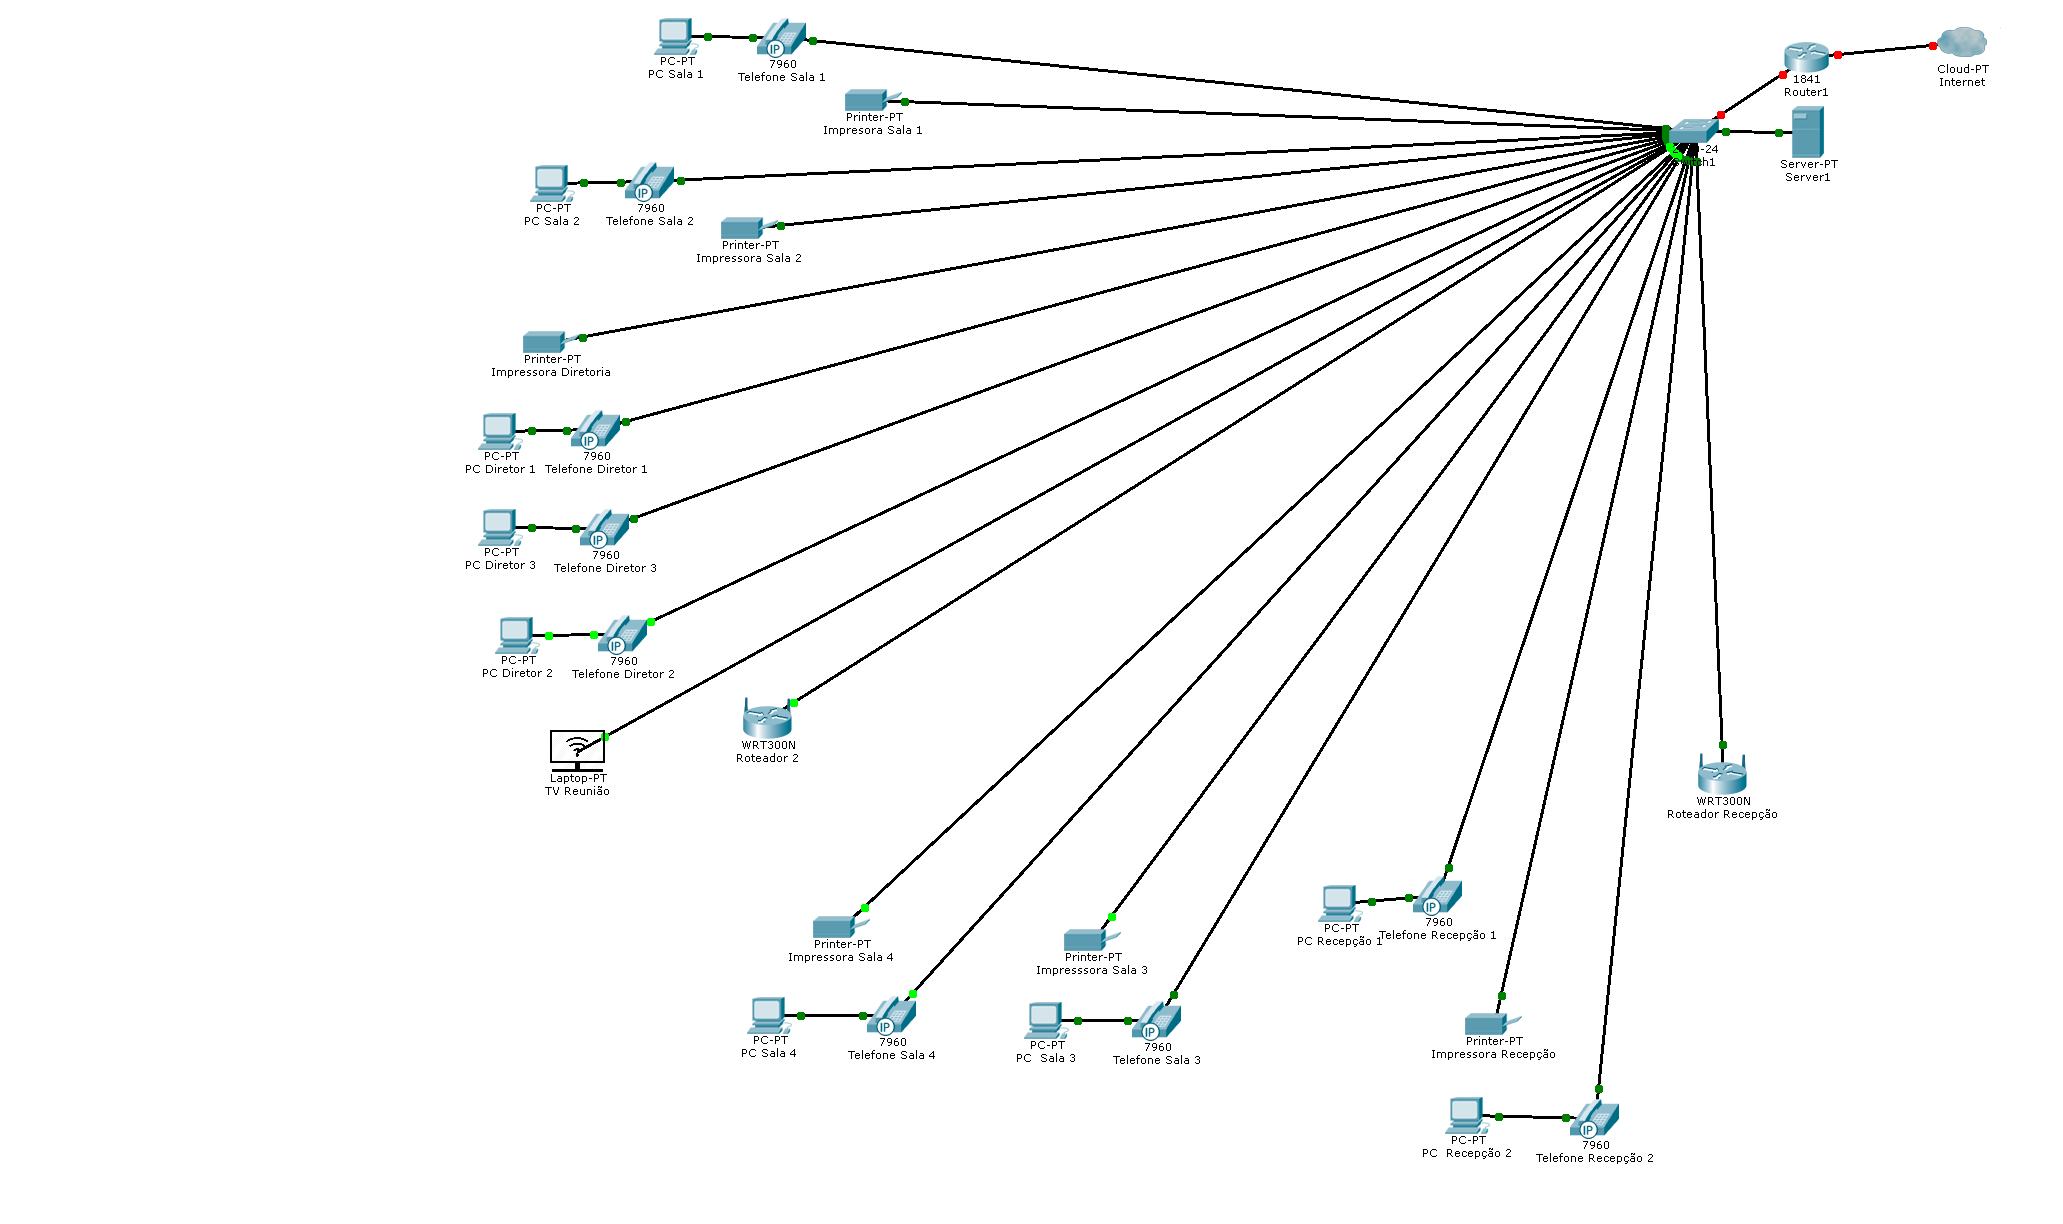
\includegraphics[]{fig2}
		\caption{Exemplo de figura sem escala}
		\label{fig2}
	\end{figure}
	
	Você pode rotacionar figuras também. Para isso utilize o parâmetro angle=-90. Repare que a escala da figura foi modificada pelo parametro height. Você também pode utilizar scale
	
	\begin{figure}
		\centering
		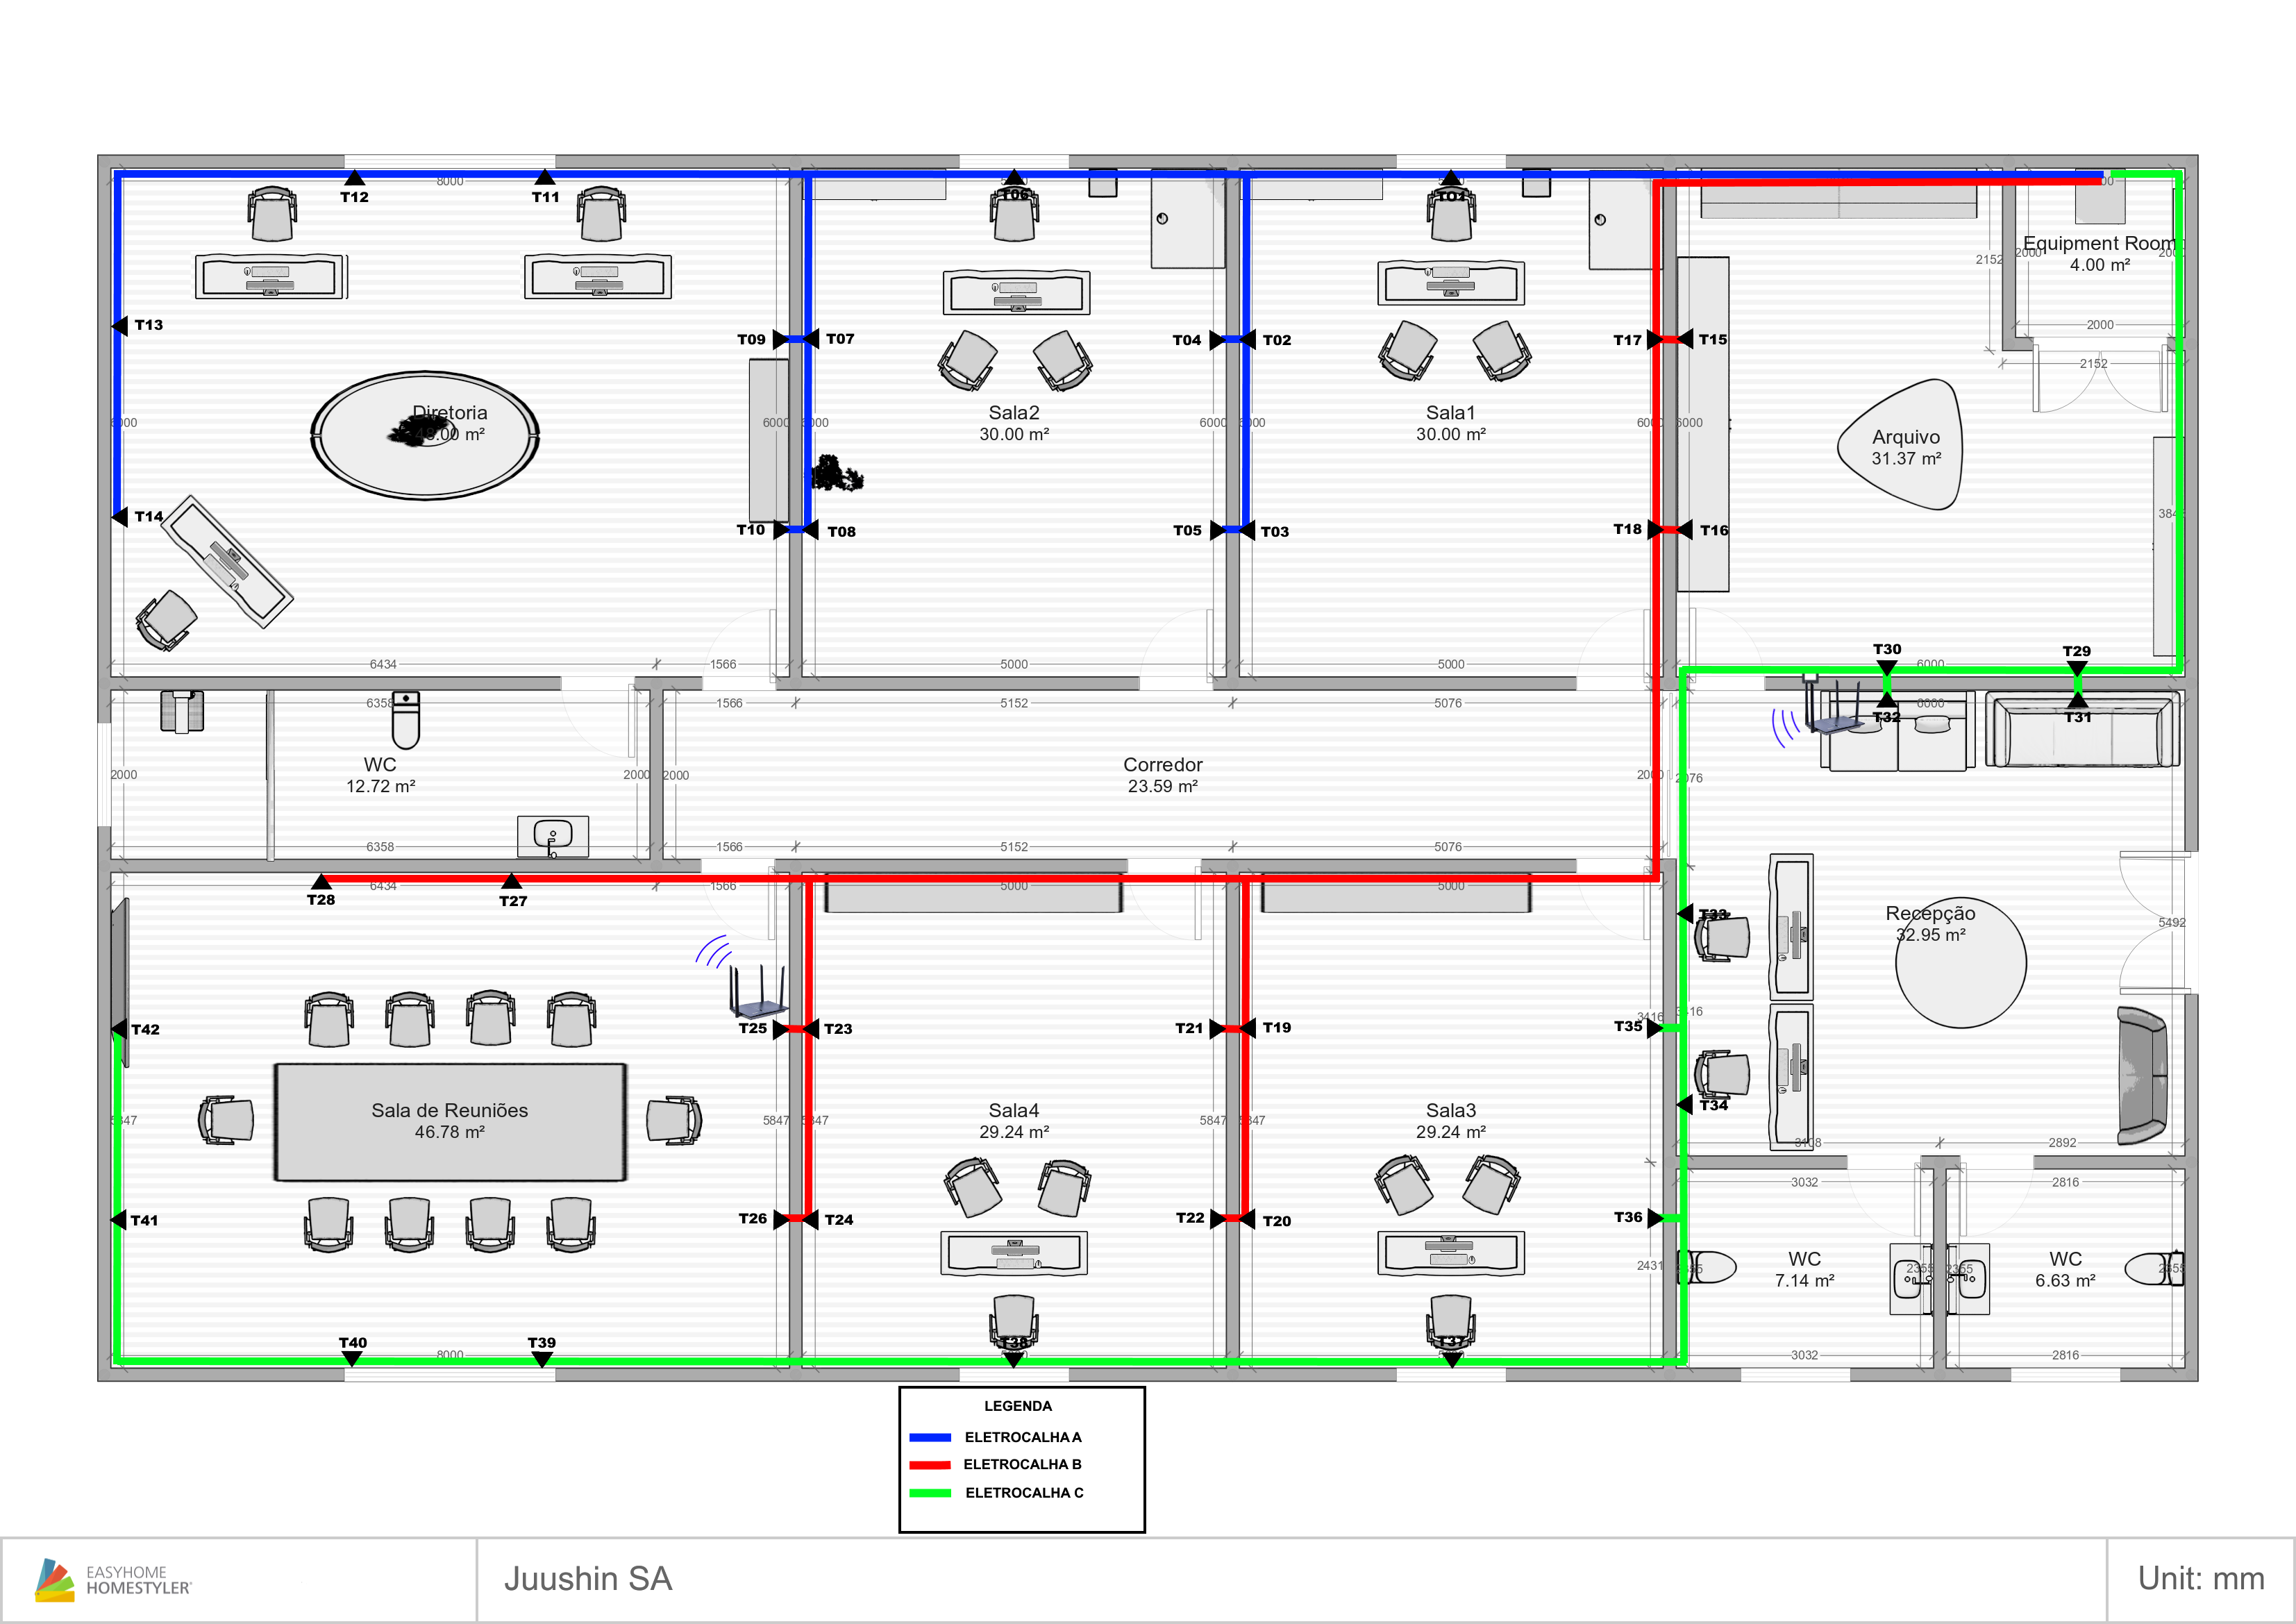
\includegraphics[height=\textwidth,angle=-90]{fig3}
		\caption{Exemplo de figura rotacionada}
		\label{fig3}
	\end{figure}
	
	\subsubsection{Resumo gráfico}
	
	Você pode optar por fazer um resumo no formato de mapa mental/conceitual. 
	Aqui foi utilizado o site https://app.mindmup.com para gerar o mapa.
	
	Para utilizar o resumo gráfico, remova o texto da seção resumo (linha 137) e inclua o código para inserir a figura, conforme figura \ref{fig4}
	
	\begin{figure}[h]
		\centering
		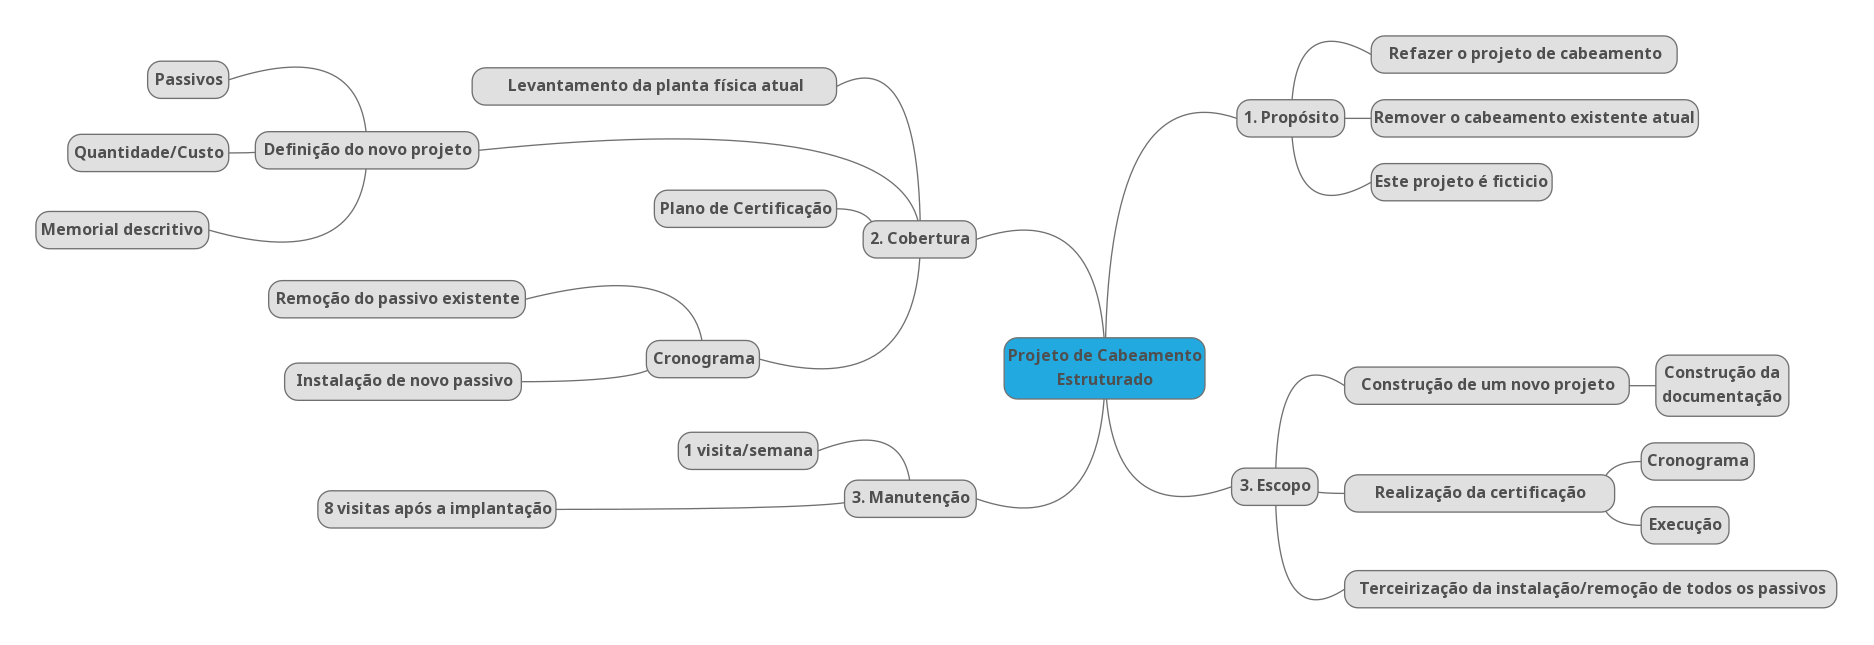
\includegraphics[width=\textwidth,height=5cm,keepaspectratio]{fig4}
		\caption{Exemplo de resumo gráfico}
		\label{fig4}	
	\end{figure}
	
	%% ***********************************************************************
	%% === ate aqui    =====  ================================================
	%% ***********************************************************************
	
\end{document}